\documentclass[12pt]{report}
\usepackage{graphicx}
\usepackage{listings}

\title{CSCI-476 Final Test}
\date{May 6, 2015}
\author{Gunnar Holwerda}
\renewcommand*\contentsname{Table of Contents}
\newcommand{\mychapter}[2]{
    \setcounter{chapter}{#1}
    \setcounter{section}{0}
    \chapter*{#2}
    \addcontentsline{toc}{chapter}{#2}
}

\begin{document}
\maketitle

\tableofcontents
\clearpage

\mychapter{1}{Executive Summary}
\section{Executive Summary}

\clearpage

% Begin Round 1

\mychapter{2}{Round 1}
\section{DiscoveredIn1655}
When starting out I was given the information that the members of mhk had been discussing RFC2100. This RFC mentions a few names, so I began using the names mentioned as subdomains of mthack.me and quickly found titan.mthack.me. I ran nmap on the host to see what ports were open.\\
	\begin{verbatim}
	$	nmap -sS -p1-65535 titan.mthack.me -v -T4
	\end{verbatim}
The nmap returned that port 22 and 23 were open. I attempted to ssh, but found that a public key was needed. Next I used telnet to connect to port 23 and was presented with my first flag ``DiscoveredIn1655''.\\
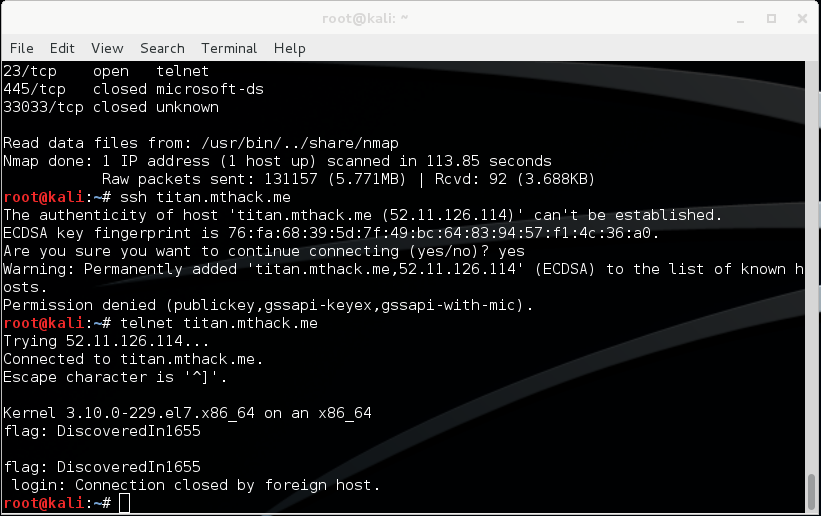
\includegraphics[scale=0.33, width=\linewidth]{img/DiscoveredIn1655.png}
\newline
\section{Th1sT1m3ItsAMoon}
In addition to titan.mthack.me, I was able to find the europa.mthack.me subdomain. After an nmap on europa I saw that port 7870 was open. There was no information about this port, so I used NetCat to connect to it, it returned ``SSH-2.0-OpenSSH\_6.6.1''. After seeing this I knew that I should use SSH to connect to europa.mthack.me on this port.
	\begin{verbatim}
	$	ssh europa.mthack.me -p 7870
	\end{verbatim}
After adding europa to my known\_hosts I was presented with my second flag ``Th1sT1m3ItsAMoon''.\\
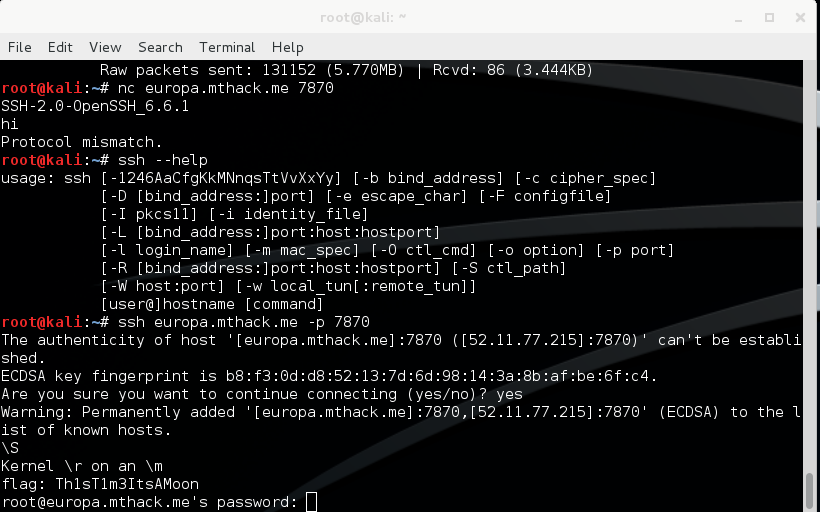
\includegraphics[scale=0.33, width=\linewidth]{img/Th1sT1m3ItsAMoon.png}
\newline

% Begin Round 2

\mychapter{3}{Round 2}
\section{SOMEFLAG}
Everything is broken!\\
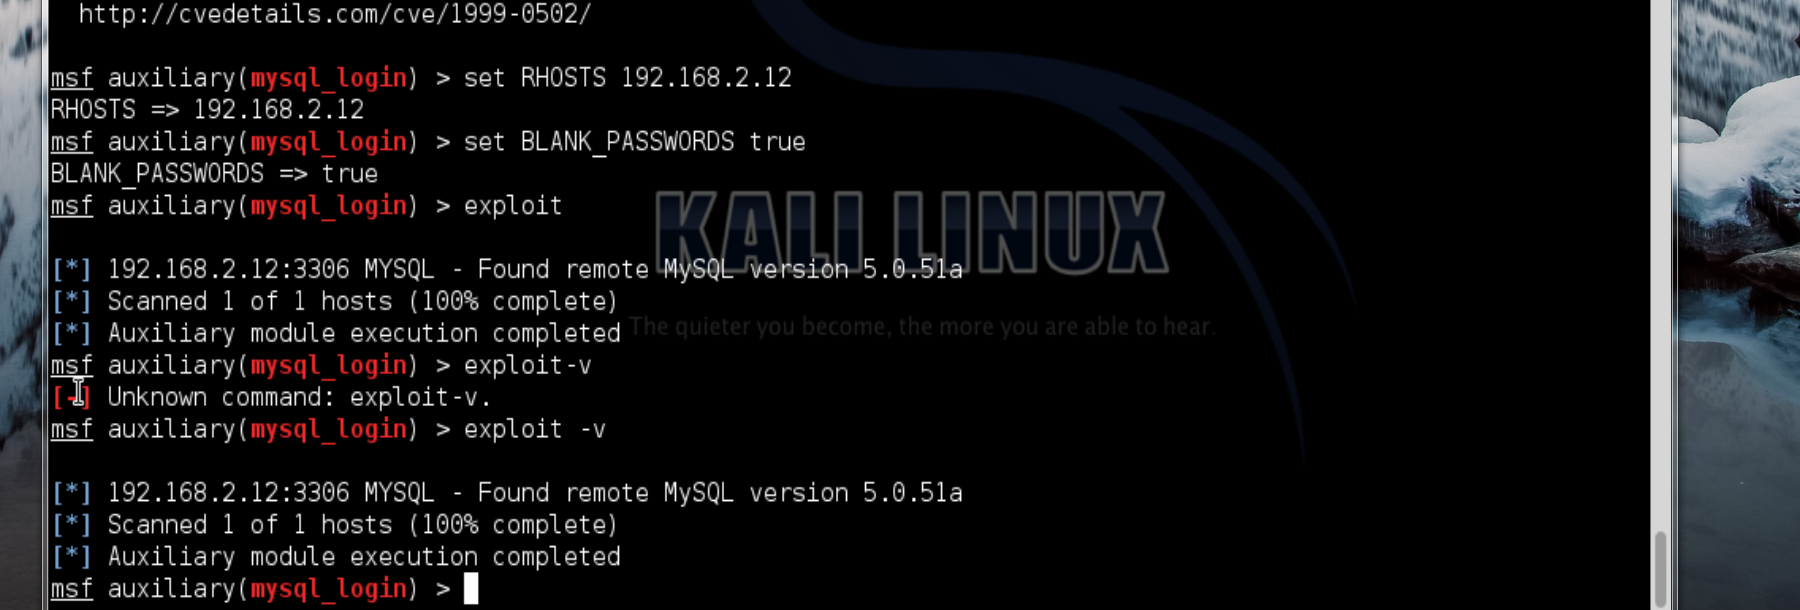
\includegraphics[scale=0.33, width=\linewidth]{blank_password_check_output.PNG}
\newline

% Begin Round 3

\mychapter{4}{Round 3}
\section{nextlevel}
Given the binary for round three, I first ran strings on the file using grep to try to find ``password'' or something along those lines. These attempts were unsuccessful, so I moved onto editing the binary using radare2. I was able to find the location of a ``jnz'' instruction right after asking for the number. I edited that instruction to be a ``jz'' instead and was presented with ``ciph3rfun.html''.\\

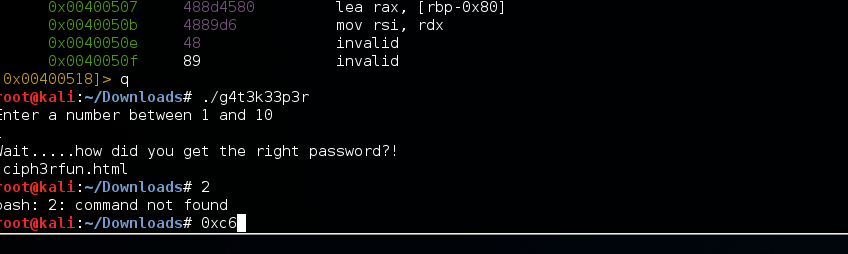
\includegraphics[scale=0.33, width=\linewidth]{img/ciph3rfunhtml.PNG}

I then visited www.mthack.me/ciph3rfun.html and was presented with some sort of enocded flag. It looked like ROT, so I went to a ROT decoder, entered the cipher text and was presented with the flag ``nextlevel''.\\
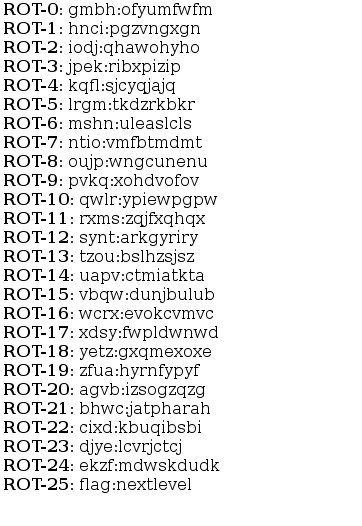
\includegraphics[scale=0.33, width=\linewidth]{img/nextlevel.PNG}

\newline
I ran a ``show grants;'' to find out how much power the user I now controlled has. Turns out I had access to everything in MySQL! What if I tried to open the ``/etc/passwd'' file?\\
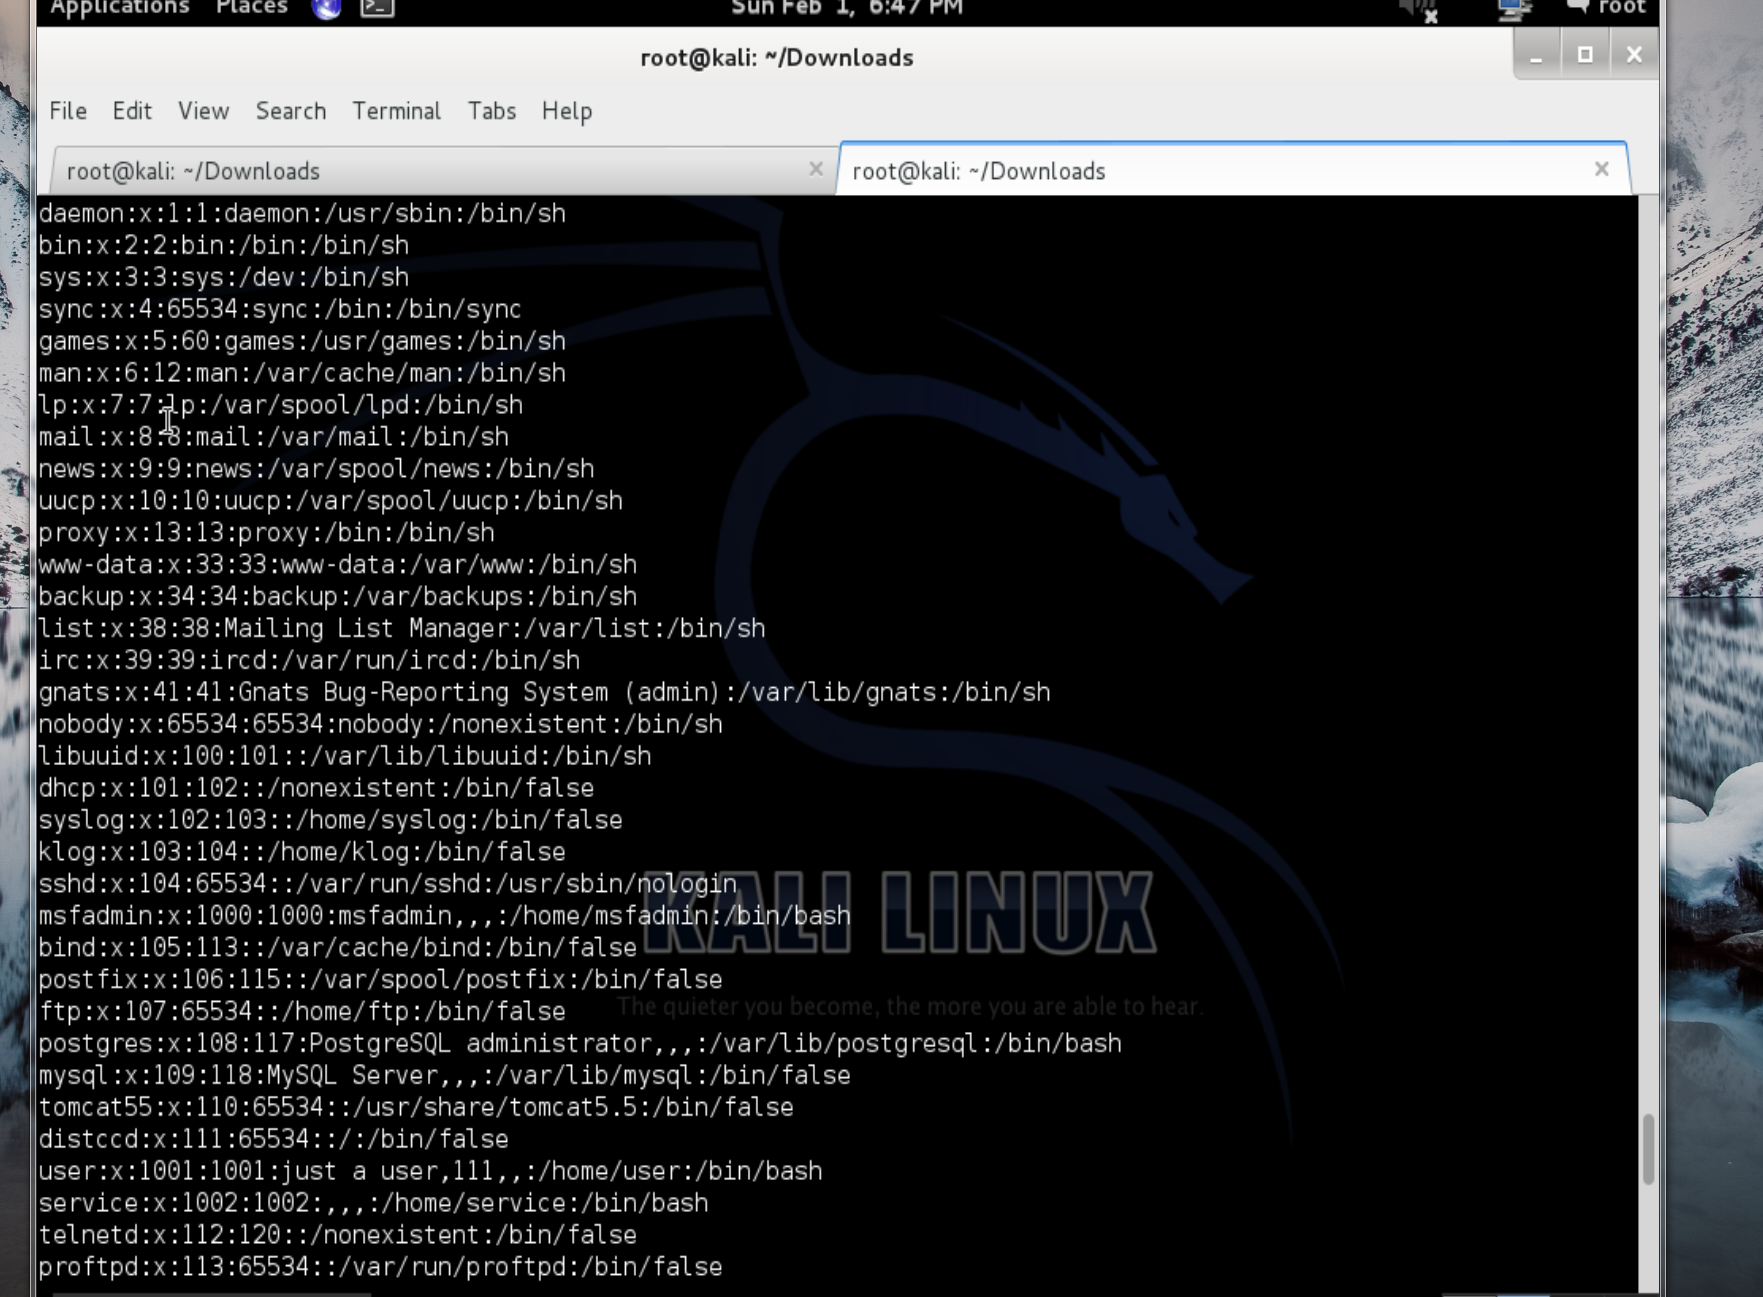
\includegraphics[scale=0.33, width=\linewidth]{_etc_password.PNG}
\newline
I was able to get the file, so now I have a list of users and what group they belong to on the system. I attempted to get the ``/etc/shadow'' file, but was rejected. So this still leaves me with no ability to get into a shell. Now I decided that I would try to investigate the datbases contained within the system to see if there was any information contained within in them that could help me out.
	\begin{verbatim}
	> show databases;
	> use mysql; 
	> Select *;
	> show tables;
	> select * from user;
	> select User from user;
	> select User, Password from user;
	\end{verbatim}
When I selected everything from the user table, I got a very messy printout of the table (see screenshot below). I was able to determine that the table contained a username and password, so I selected both of those from the table. Unfortunately the passwords were not in the table.\\
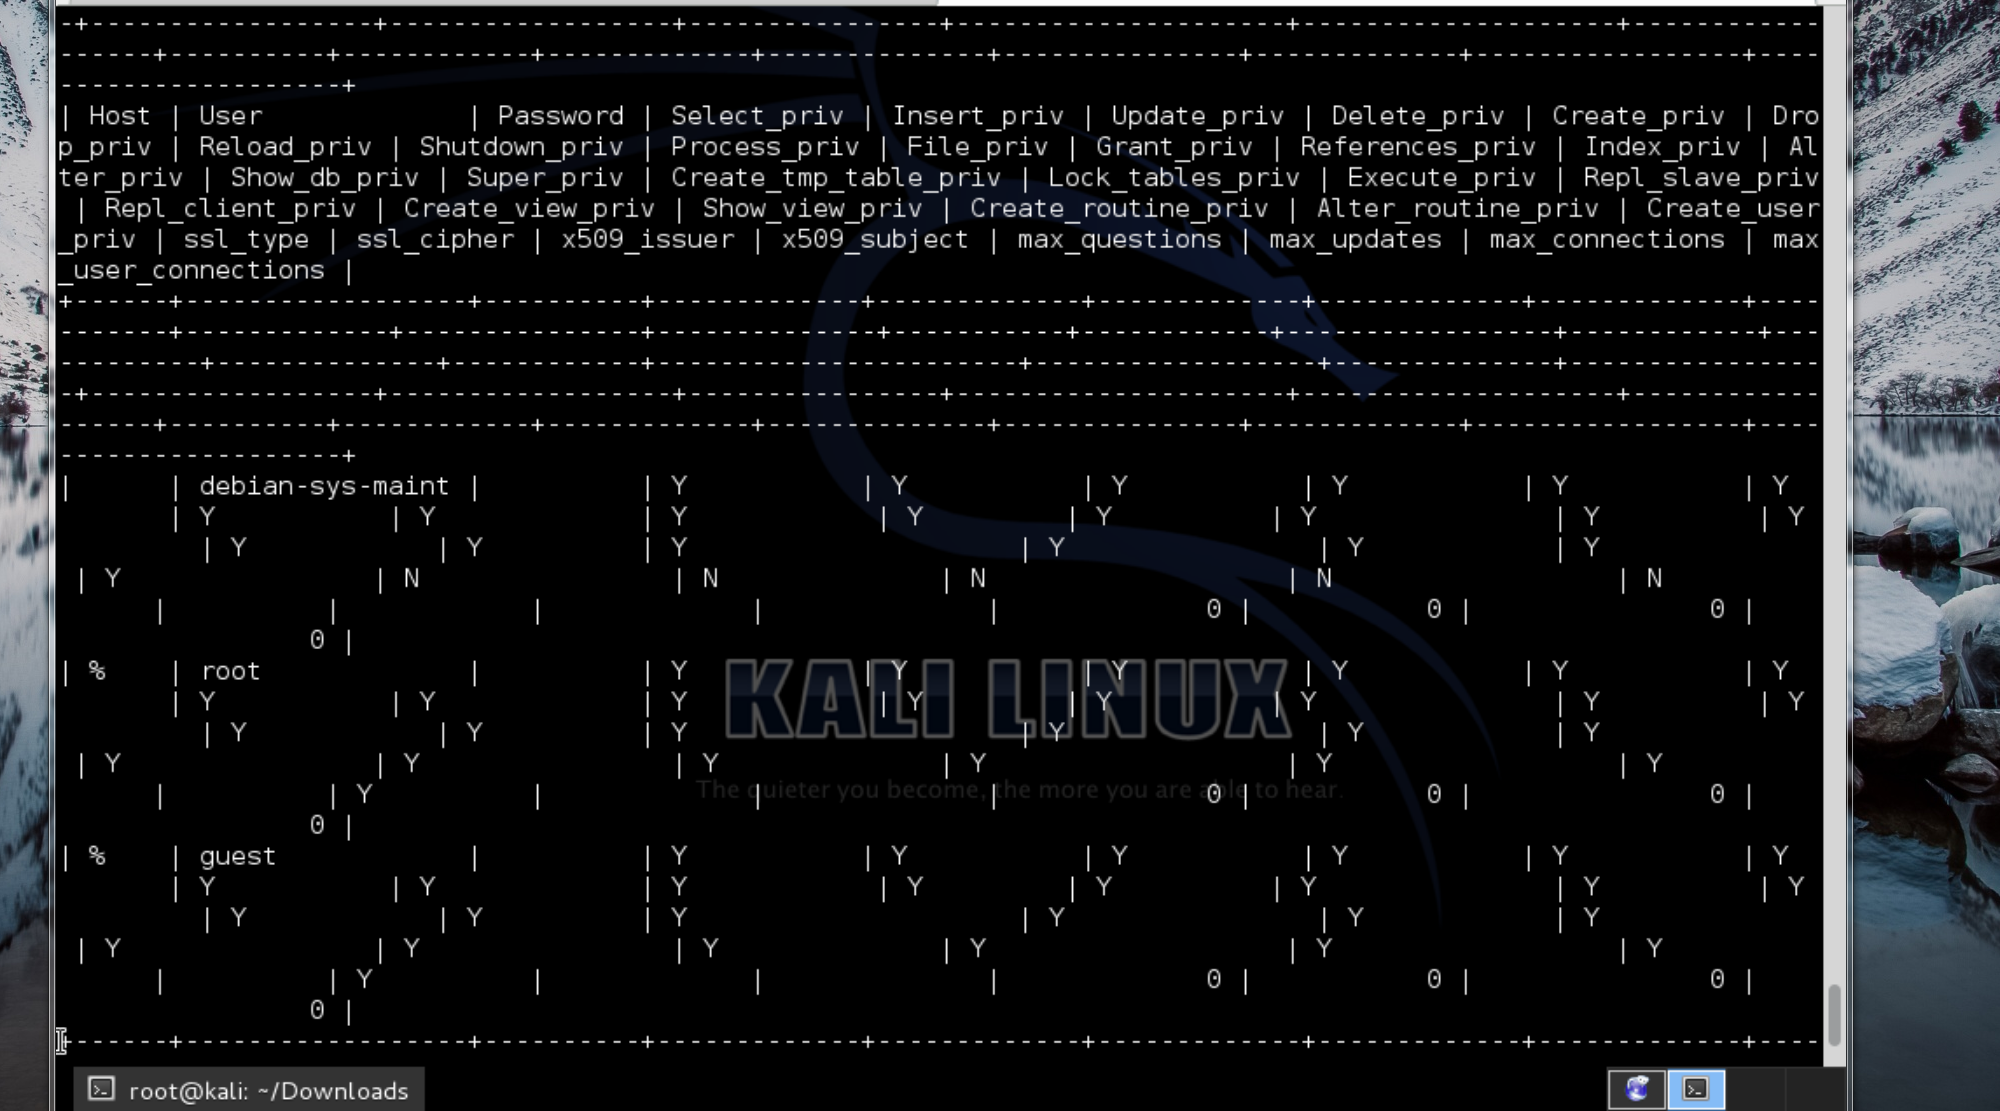
\includegraphics[scale=0.33, width=\linewidth]{weird_output.PNG}
\newline
I then attempted to try to use the mysql\_hashdump tool from msfconsole, unfortunately it was unable to provide me with anything. Next I decided to see if there were any known exploits for the current MySQL version that was running on the system. That search turned up nothing as well. I went into MySQL again and grabbed the print out of the ``/etc/passwd'' file from before to use it as a user list to try to brute force an SSH account.
\newline

% Begin Round 4

\section{5}{Round 4}
I determined that I was going to try to brute force an SSH account using the users from the ``/etc/passwd'' file I was able to print out from MySQL. AFter waiting for a long time as Hydra attempted to test multiple passwords for the large user list, I decided to just focus on one user. I picked the user ``user'' and decided to try to brute force it using the namelist.txt wordlist from ``/usr/share/wordlists/metasploit/'' built into Kali. 
	\begin{verbatim}
	# hydra ssh://192.168.2.12 -l user -P /usr/share/wordlists/metasploit/namelist.txt -v -t 8
	\end{verbatim}
\includegraphics[scale=0.33, width=\linewidth]{find_the_login.PNG}
\newline
I was able to successfully find the password for ``user'' and thus login to an SSH account with shell access.
\clearpage

\mychapter{6}{Summary}

\clearpage

\mychapter{7}{Biography}

\end{document}